\subsection{Cen�rio}

O uso da realidade aumentada em manuten��o de aeronaves pode trazer ganho no que
tange fornecer informa��es de procedimentos ao mec�nico ou mesmo previs�o de
falhas ou reconhecimento de regi�es com falha.

 Como caso de uso ser� adotado a janela de inspe��o frontal como mostrado na
 imagem~\ref{fig:ERJ190} que mostra onde fica localizado na aeronave Embraer
 190. 
 
\begin{figure}[h!]
\centering
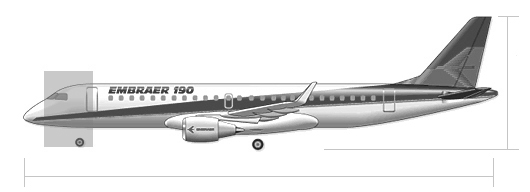
\includegraphics[scale=0.8]{images/ERJ190}
\caption{Posicionamento da LRU}
\label{fig:ERJ190}
\end{figure}


Foi selecionado um objeto sem texturas e com material brilhante, na janela de
inspe��o por sofrer mais influ�ncia em
varia��o de ilumina��o e ser �nico na janela de inspe��o em quest�o.